\chapter{Python~编辑及运行环境配置}
在本课程中,我们选择安装anaconda这一Python发行版进行学习与开发。一方面是因为anaconda在安装时不仅仅能够安装一个python解释器,
其也会同时安装ipython kernel,Jupyter notebook,matplotlib,scipy,numpy等多个常用的(也就是本课程中会用到的)第三方库。另一方面,anaconda提供Spyder这一高集成度,
便于初学者学习和调试的IDE,可以提供给我们“开箱即用”的体验\footnote{anaconda本身也提供很多别的功能,本章节后面会进行简要介绍}。

如果你想要挑战自己,当然可以自行到Python项目官网\footnote{https://python.org}上自行下载和安装Python解释器,而后使用pip包管理工具安装
我们所需的各类第三方库或者第三方组件(包括Spyder,也可以通过pip来自动安装)。但在正式开始教程之前,需要强调,作为初学者,请不要同时安装
纯净Python解释器和anaconda,即不要
让使用下载的Python安装包所安装的python解释器同anaconda在同一台电脑上并存,因为此时你的电脑里将同时有两个python运行环境,且这两个运
行环境没有通过环境管理器进行管理,其激活次序,即运行python脚本文件时正在使用的python解释器,或是尝试使用pip安装第三方库所指向的环境不易明确。
总之,作为课程的初学者,也是本手册后面的安排,我们将基于anaconda(conda+python解释器)进行介绍,包括环境配置,工具使用等,
所有代码也将会在这个环境下进行运行。

本章节,我们将会介绍Anaconda的下载与安装过程,Spyder的基本使用方法,并在最后简要介绍conda环境管理工具和pip包管理工具的使用。
\section{Anaconda的下载与安装}
\subsection{Anaconda下载与安装}
Anaconda现已实现完善的公司化运营,可以访问其网站下载Anaconda:

https://www.anaconda.com/download

但通常,出于下载速度的考量,我们选择使用校园网联合镜像站的方式下载Anaconda,这不仅仅可以提供更快的安装包下载速度,同时其分发的
安装包也会将其中的默认镜像站替换成自己的分发站点,从而提供更高的pip与conda下载与更新速度。提供镜像站的组织有很多,如清华大学TUNA协会,中国科学技术大学所等高校及高校学生组织
所提供的下载源,此处以清华大学TUNA协会提供的下载源为例。

访问https://mirrors.tuna.tsinghua.edu.cn/anaconda/archive/ \footnote{此为双栈站点,可以自动选择IPv4或IPv6解析,将mirrors替换为mirrors6则只解析IPv6,替换为mirrors4则只解析IPv4,在校园网环境下,使用IPv6下载的文件不计流量。},
获取anaconda安装包列表。根据自己的操作系统版本和硬件架构,选择
下载对应的安装包体(如Windows-x86\_64对应AMD,
Intel处理器的Windows设备,MacOSX-arm64对应搭载Apple Silicon M1、M2、M3的设备)。
在当前的时间节点,建议选择Anaconda3-2023.09开头的安装包。如图\ref{fig:anacondaSelection}所示
\begin{figure}[htbp]
    \centering
    \includegraphics*[width=0.8\linewidth]{pic/tuna_anacondaDownload.png}
    \caption{Anaconda3安装包示例}
    \label{fig:anacondaSelection}
\end{figure}

对于不太熟悉命令行操作的同学来说,建议下载文件拓展名为pkg或exe的安装包,其可以提供图形化的安装界面和选项。具体安装过程在此不再赘述,
但请注意,\textbf{不要}把Anaconda安装在\dotuline{含有中文的目录}下,尤其注意你的Windows用户名是否带有中文。如果你不确定,可以直接将其安装在C盘外的其
他盘符\footnote{不要将Anaconda安装在C:/Program Files中},另外创建的文件夹中。

\subsection{环境变量配置}
配置环境变量的目的是令其他程序在运行python时能够直接找到base环境下的python,而不需要手动指定,同时也方便我们直接打开命令行就可以直接使用python解释器运行和调试程序。
anaconda提供了方便快捷的命令行环境的环境变量配置方式,只需要切换到conda.exe的安装
位置\footnote{windows下的默认位置C:\textbackslash Users\textbackslash 用户名\textbackslash anaconda3\textbackslash Script,macOS下的默认位置/Users/用户名/anaconda3/bin},直接
在命令行中运行{\texttt{conda init}}即可\footnote{对于powershell,需要使用\texttt{.\textbackslash conda init}}。运行效果如图\ref{fig:condaInit}所示。
\begin{figure}[htbp]
    \begin{minipage}[t]{0.4\linewidth}
        \centering
        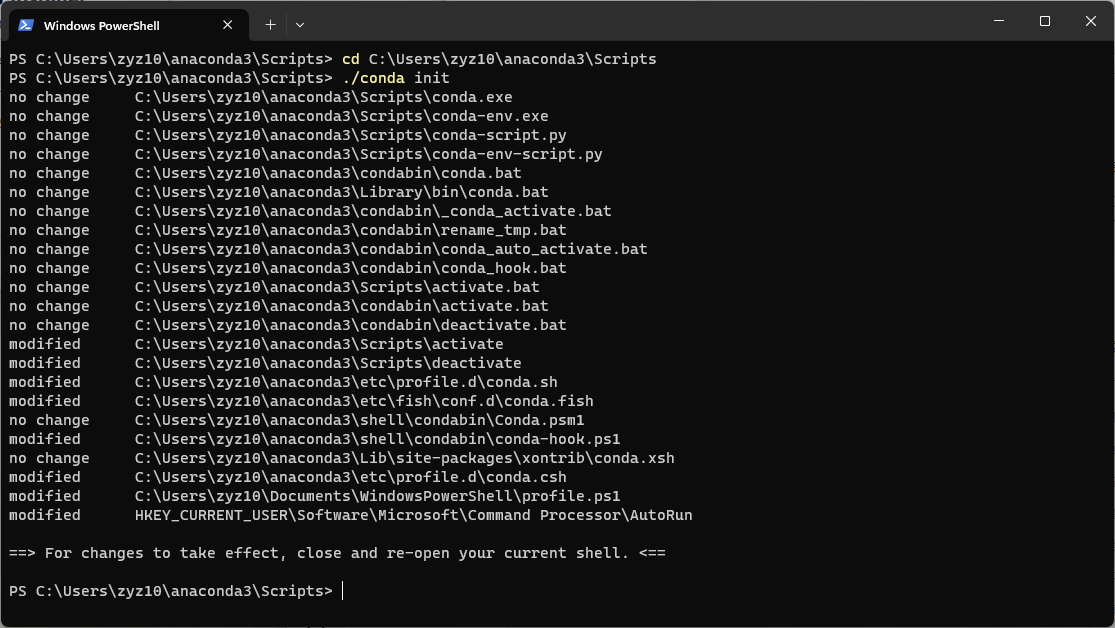
\includegraphics[height=0.5\linewidth]{pic/conda_init_windows.png}
        Windows
    \end{minipage}
    \hfill
    \begin{minipage}[t]{0.4\linewidth}
        \centering
        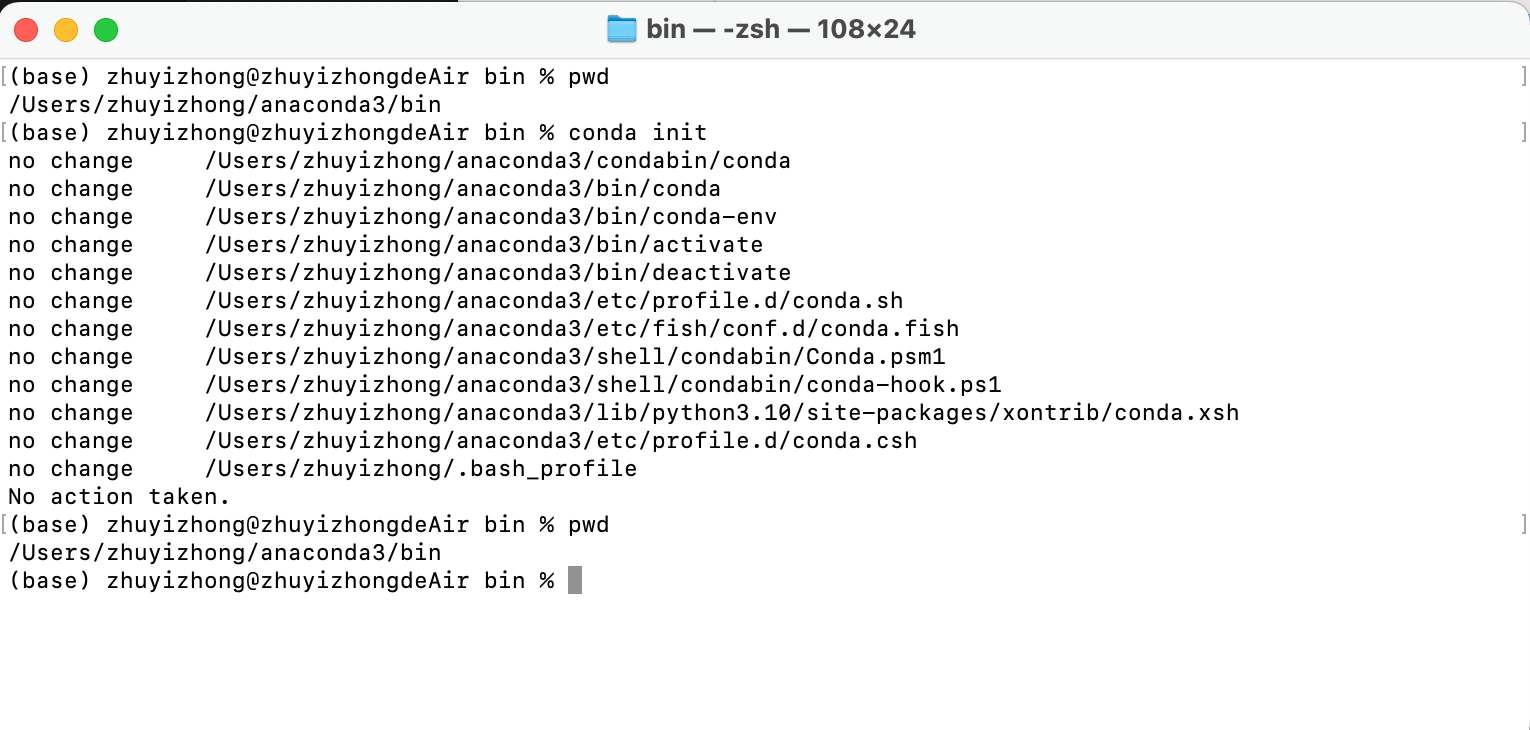
\includegraphics[height=0.5\linewidth]{pic/conda_init_macos.png}
        macOS
    \end{minipage}
    \hfill
    \caption{使用~conda init~自动配置环境变量的结果}
    \label{fig:condaInit}
\end{figure}

而后,重新打开命令行(Windows 10/11中的终端\footnote{打开powershell时如果出现异常报错,则需要使用Win+X点选终端(管理员)打开powershell,运行Set-ExecutionPolicy RemoteSigned以使能脚本运行功能},macOS中的控制台),可以看到在命令前面出现了(base)字样,表明当前激活的python环境是conda管理的base环境。

\subsection{Spyder使用}
安装流程结束后,在开始菜单(macOS:启动台)中寻找到Anaconda-Navigater,点击运行。
加载结束后,可以打开Spyder,如图\ref{fig:navigater}所示
\begin{figure}[htbp]
    \centering
    \includegraphics*[width=0.7\linewidth]{pic/anaconda_nav_Spyder.jpg}
    \caption{Anaconda Navigater主界面}
    \label{fig:navigater}
\end{figure}

下面介绍Spyder主界面各面板的功能。但在开始之前,我们先来把Spyder的界面语言修改成中文。点选 
Tools-Preferences 打开选项页面,而后在Application-Advanced settings中找到Languages,选择简体中文即可。如下图所示
\begin{figure}[htbp]
    \begin{minipage}[h]{0.3\linewidth}
        \centering
        \includegraphics*[height=0.3\linewidth]{pic/Spyder_Language_1.png}
    \end{minipage}
    \hfill
    \begin{minipage}[h]{0.6\linewidth}
        \centering
        \includegraphics*[height=0.4\linewidth]{pic/Spyder_Language_2.png}
    \end{minipage}
\end{figure}

下面介绍Spyder主界面各面板的功能与作用。设置中文并打开Spyder后,初始界面如图\ref{fig:spyderMain}所示。
\begin{figure}[htbp]
    \centering
    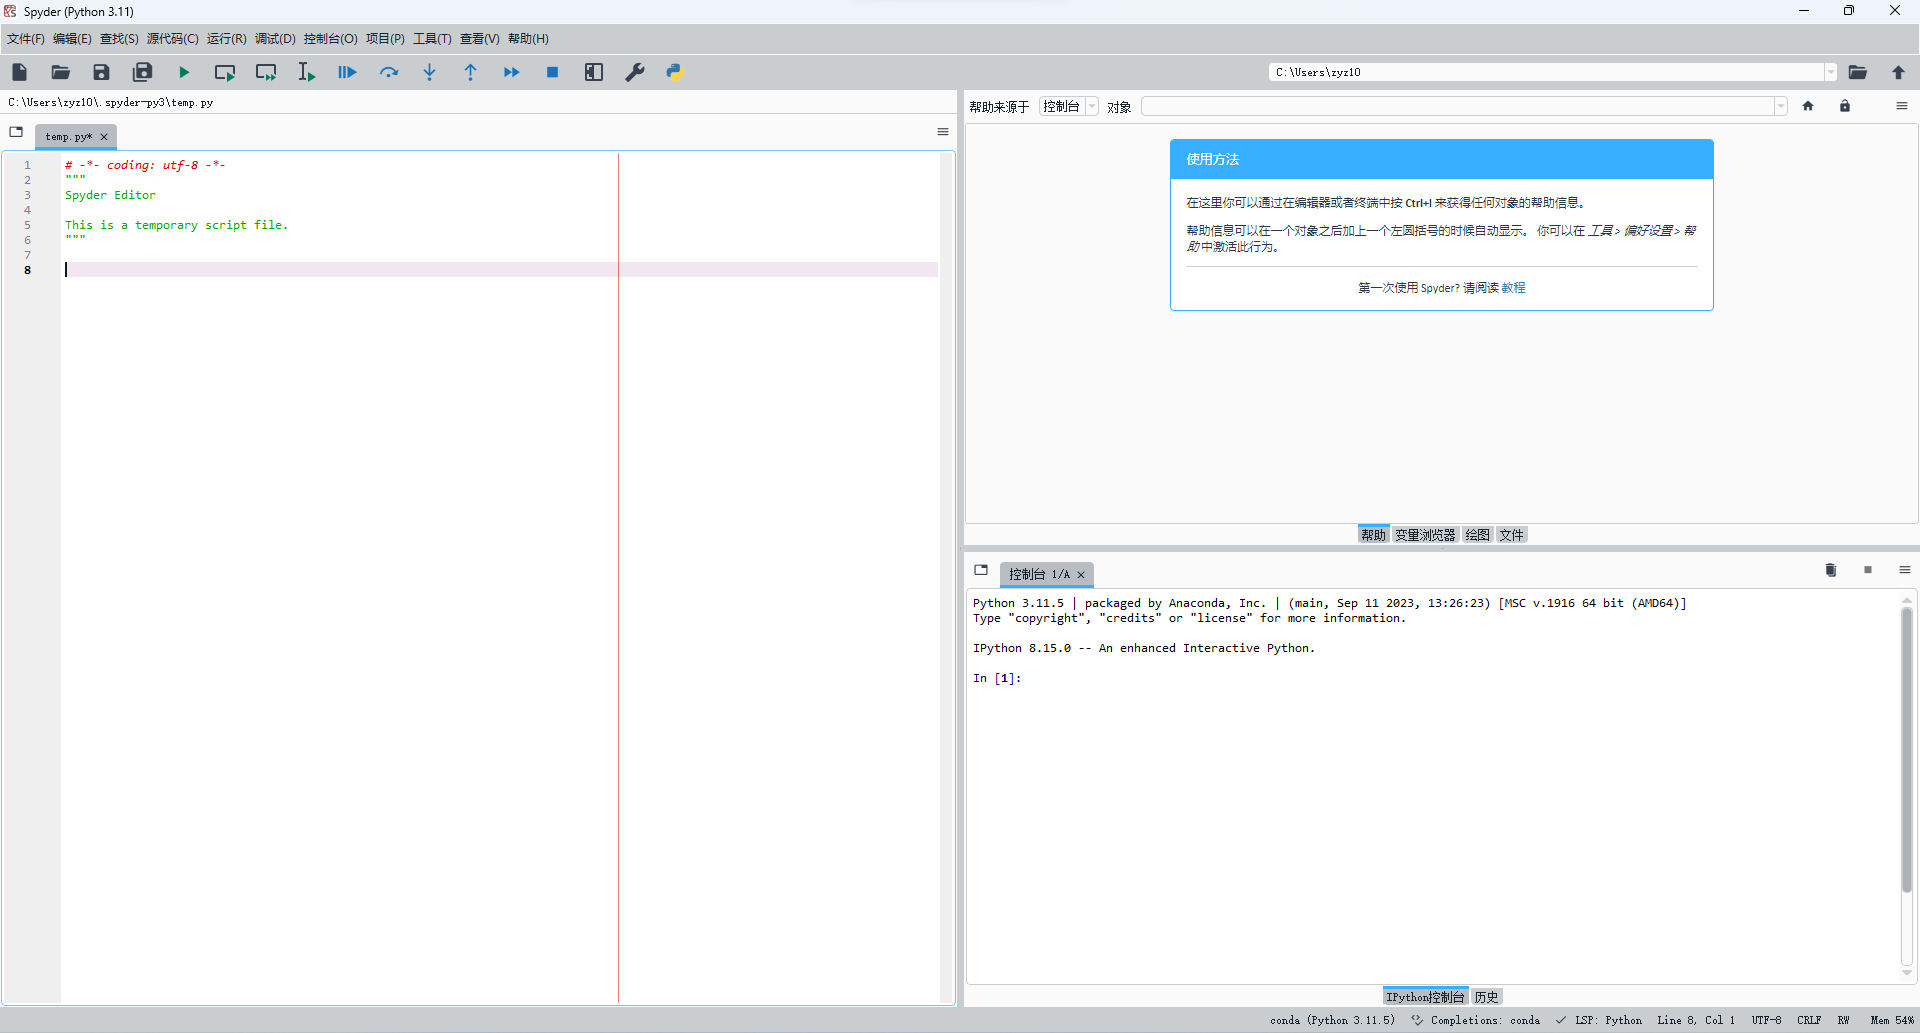
\includegraphics[width=0.7\linewidth]{pic/spyder主界面.png}
    \caption{Spyder 主界面}
    \label{fig:spyderMain}
\end{figure}